\documentclass[main.tex]{subfiles}

\begin{document}

\section{Scope of thesis and Contributions}


\section{Offer Network Specifciation}

\begin{figure}
  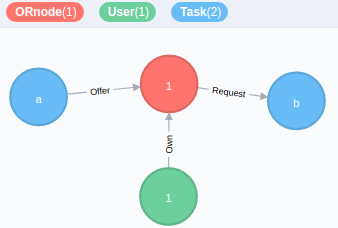
\includegraphics[]{example1.png}
  \caption{User 1 uploads an ORnode to offer task a and requests task b in exchange.}
  \label{example1}
\end{figure}

\begin{figure}
  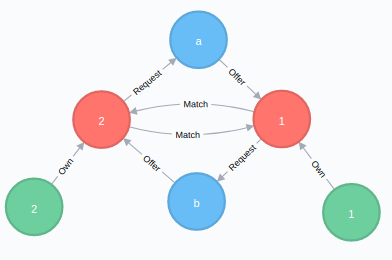
\includegraphics[]{example2.png}
  \caption{User 2 uploads an ORnode to offer task b and requests task a in exchange.
           \\Now there is a cycle/match.}
  \label{example2}
\end{figure}

An \textbf{offer network} instance can be formally modeled as a directed graph, $G$, where vertices $t \in T$ represent tasks, $u \in U$ users, and labeled directed edges $(t_a,t_b) : u_1$\footnote{Can be a hypergraph if one wants user nodes rather than labels.}\footnote{In the current implementation, actually a multigraph: there can be multiple edges ($t_a,t_b$).} represent an offer by user $u_1$ to do task $t_a$ in exchange requested task $t_b$. See Figure \ref{example1}. Due to implemention details in Neo4j\footnote{\url{https://neo4j.com/}}, I create (offer, request) nodes for labeled directed edges, which I call \textbf{ORpairs}. I will call this the task-centric graph formulation.

A matching of users who can satisfy each other is a vertex cycle. See the simplest case below in Figure \ref{example2}. However, there is no guarantee users will be satisfied with the proposed match. I make the simplifying assumption that there is a global match acceptance probability $p$, that is, it is uniform and independent\footnote{Moreover, Dickerson \cite{Dick} notes this assumption can also protect users, such as badly sick patients, from being marginalized.}.

\subsection{Task and ORnode Distribution of Graph}
The more realistic the underlying graph model, the better the experiments will be. However, there is no guarantee the distribution of goods and services in an offer network will resemble those on eBay, social networks, the internet, or regular markets.

A basic defendable assumption is that the graph will be scale-free: a few task will be very popular and others unpopular. There will likely be some differnce in popularity to \textit{offer} and to \textit{request} tasks, but not that much. I modified a graph generator in NetworkX \cite{netX} to generate such graphs, described in by \cite{Bol}. In my modification the model generates a set number of edges and for each edge adds a new task with probability $\alpha + \gamma$.

Also worth mentioning on this note is a user-centric study of the eBay graph \cite{ebay}\footnote{The data is obtained via crawling eBay feedback.}. They noted the following properties on eBay:

\begin{itemize}
  \item Skewed degree distribution: i.e., there are a few big sellers.
  \item Dissasortativity: users tend to buy and sell different types of products.
  \item Linear preferential attachment in terms of positive feedback.
     \\ Strong aversion avoidance of users with negative feedback.
  \item Densification over time.
  \item No rich club connectivity (basically because big nodes are mass sellers).
\end{itemize}

These observations generally agree with the basic assumption made for the graph model, and imply that there will be little task-centric clustering of ORnodes.


\subsection{Dynamic Offer Network Specification}
The dynamic offer network starts with a scale free graph generated as above with $N^o_0$ ORnodes and $N^u_0$ users and each time-step $t$, $n^o$ and $n^u$ new ORnodes and users. Each step there are $(\alpha + \gamma) n^o$ new tasks added to the network every step. The experiment is run until $N^o_m$ ORnodes have been added. Between each step matchings are suggested, processed (by users), and accepted ORnodes are removed from the graph.

It is possible to make $n^o$ and $n^u$ depend on $N^o_t$, $N^u_t$, on each other, or be drawn from a probability distribution.

\subsection{Cycle Size and Acceptance Probability}

\subsubsection{Motivation}
The optimal solution clearly depends on acceptance probability, primarily biased by the optimal cycle size. In general, finding a maximum edge-disjoint cycle cover with cycle-weights (to account for acceptance probability) is NP-hard \cite{Bir}, so the prefrred algorithm may depend on the current estimation for $p$. If near $1$, (near) unlimited cycle sizes are welcome; if low, 2-exchanges will always be preferable.  In the middle, an algorithm may want to choose cycles with greatest expected value.

Below I include some basic probabilistic anlaysis to find out how high is high and how low is low.

Similar analysis is done by Dickerson \cite{Dick} \cite{Dick3}; however, Dickerson uses an optimal solver and pays less attention to determining heuristics.

\subsubsection{Analysis}

In a cycle $c$ of size $k$, the probability of acceptance is $p_k = p^k$.

Thus the expected number of satisfied users is: $\E[c_k] = k p^k$. For a given $p$, the best cycle size is given by $k = -\frac{1}{\ln p}$, and the best attainable for $p$ is $-\frac{1}{e \ln p}$.

\begin{figure}
  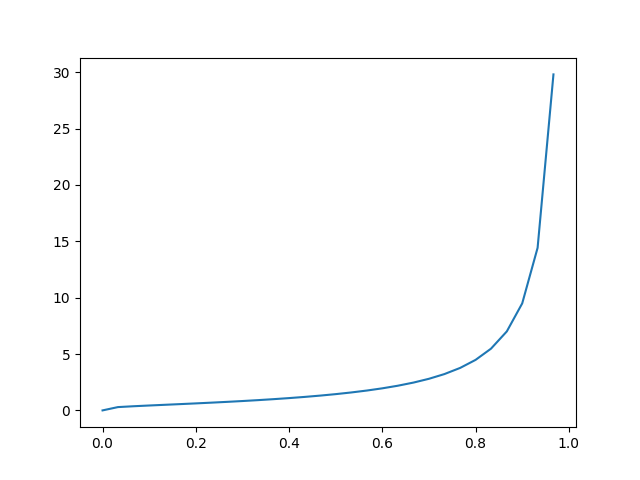
\includegraphics[scale=0.65]{best-k.png}
  \caption{Best k-cycle for p from 0.8 to 1}
  \label{best-k}
\end{figure}

\begin{figure}
  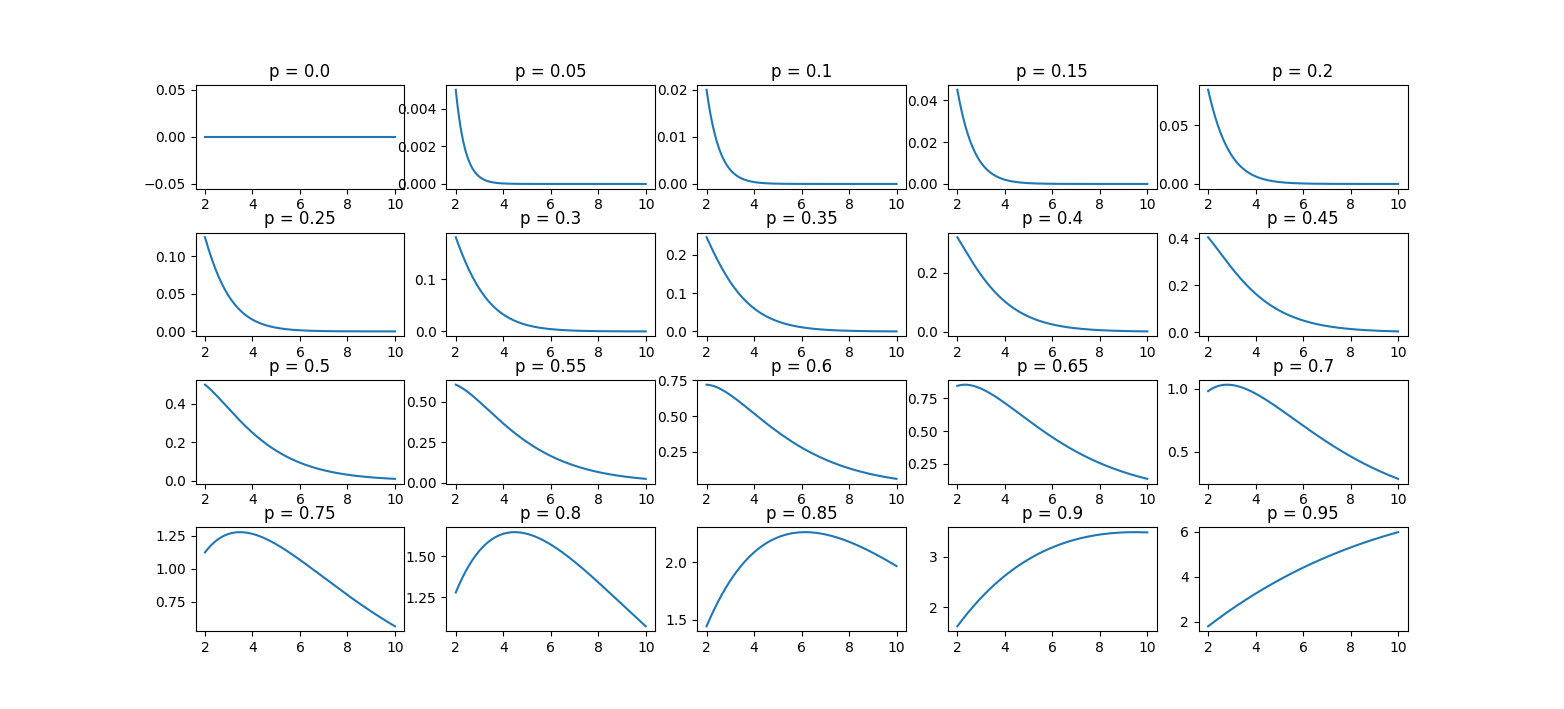
\includegraphics[width=\textwidth]{eckp1.png}
  \caption{$\E[c_k]$ for $k = 2 \dots 10$}
  \label{eckp1}
\end{figure}

\begin{figure}
  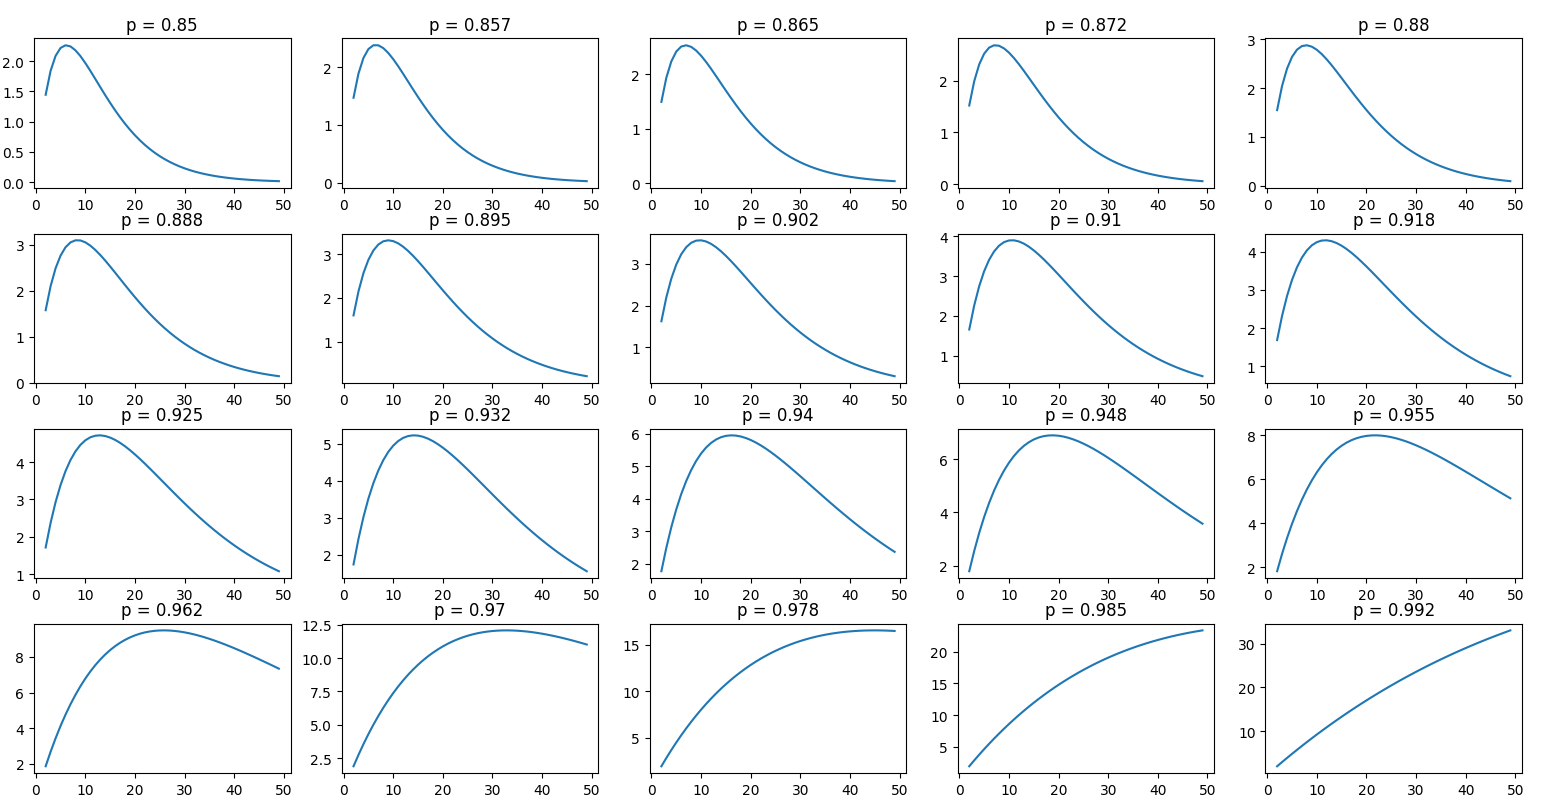
\includegraphics[width=\textwidth]{eckp2.png}
  \caption{$\E[c_k]$ for $k = 2 \dots 50$}
  \label{eckp2}
\end{figure}

As can be seen in Figure \ref{best-k}, the optimal cycle size exponentially incresaes for $p > 0.95$ ($k \approx 19.5$), so the maximum without cycle-length constraints will likely suffice. And in Figure \ref{eckp1} one sees that $2$-cycles are optimal $p < 0.7$. The Polynomial time solution is less clear for the following cases:
\begin{itemize}
  \item $0.7 < p < 0.85$ where $ 2 < k < 10$ is optimal.
  \item $0.85 < p < 0.95$ where $ 10 < k < 30$ is optimal,
      \\yet the larger cycles are little bitter than shorter ones.
\end{itemize}

For human users without very specific task formulations, $p$ likely lies in this range.

\subsubsection{How many matches are needed to for acceptance?}
There is an approach\footnote{The hanging ORnode approach is discussed in the Algorithms section.} to make long-cycles more feasible with moderate $p$ where a match can be accepted so long as both of its neighbors in a cycle accept the match as well. Thus we are interested in how many times a user needs to be matched before getting a satisfactory match.

In a given round, the probability the suggested match goes through is $p^3$ as both neighbors in a cycle also need to accept. Thus the expected number of rounds for acceptance follows the geometric distribution: $\sum_{k=0}^{\infty} k p^3 (1 - p^3)^{k-1} = \frac{1}{p^3}$.

\begin{figure}
  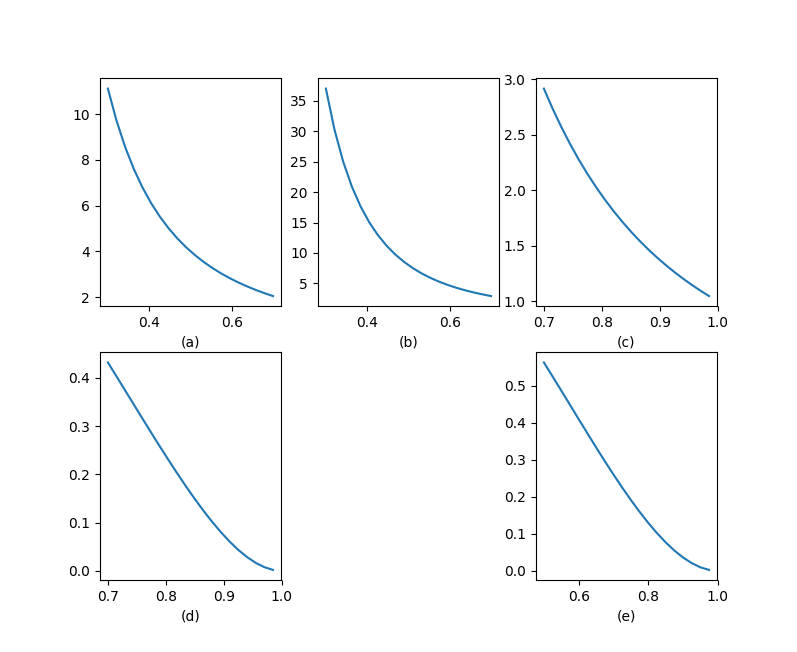
\includegraphics[width=\textwidth]{nrounds.png}
  \caption{(a)-(c) plot expected number of rounds for acceptance of an ORpair for different $p$. (a) is for 2-cyles. (b) and (c) k-cycle. (d)-(e) plot the probability of an ORpair not being accepted in 2 rounds. (d) is k-cycle and (e) is 2-cycle.}
  \label{nrounds}
\end{figure}

As one can see in Figure \ref{fig:nrounds}, one expects 5 rounds to be needed by $p = 0.6$. Fortunately, for $p > 0.7$, one expcets less than 3 rounds to be needed. With 2-cycles, one only needs 3 or 4 rounds for $p = 0.6$ or $0.5$. For lower $p$, the offer network will likely be too frustrating for human users: matching will have to be done on more detailed task specifications \footnote{Acceptance probaility is likely proportional to how detailed task specifications are; however, there are also limits as to how detailed humans can be.}.

One can also easily calculate the probability acceptance for an ORpair will take more than two rounds: $1 - (p^3 + p^3 * (1 - p^3))$.

\subsubsection{Application to Kidney Exchange}
When exchanging kidneys there is a type of incompatibility not checked prior to initial matching: PRA (percent reactive antibody). Roth et al. \cite{Rot2} split the distribution into low, medium, and high PRA with respective 5, 45, and 90 percent probability of positive crossmatch (rejection). The frequency among kidney donors is 70, 20, and 10 percent. Thus for 10 percent of matches, anything but 2-way has very low expectation, and for another 20 percent, 2-way is still expected to perform twice as well as 4-way matches. For the remaining 70 percent, however, 20-way matches are best, and 50-way still preferable to anything less than 10-way matches.

Thus when mixing low, medium, and high PRA the result of 2-way and 3-way matches being almost as good as unconstrained is unsurprising. This also seems to be a result of there only being 4 blood types, and thus no benefit to $(>4)$-way matches \cite{Rot2}.

Morevore, Dickerson \cite{Dick} \cite{Dick3} calculates acceptance probabiltiy\footnote{Optimistically based on only positive crossmatch.} to be at most $30$ percent: that is, 2-way matches always preferable to 3-way.

\subsection{Additional Features}

Below is a list of potentially desirable features of an offer network that don't qualify for an MVP:
\begin{itemize}
  \item Reputation biased matching
  \item Preferences for matching based on
    \begin{itemize}
      \item User preferences
      \item Task prefreences
    \end{itemize}
  \item ORs and ANDs of offers or request
  \item Task categories for hard/soft constraints
    \begin{itemize}
      \item Similarity based task-grouping
    \end{itemize}
\end{itemize}


\end{document}


%% For loading example graph into Neo4j
%%CREATE (t1:Task {id:'a'})
% CREATE (t2:Task {id:'b'})
% CREATE (u:User {id:'1'})
% CREATE (u2:User {id:'2'})
% CREATE (o:ORnode {id:'1', offer:'a', request:'b', user:'1'})
% CREATE (o2:ORnode {id:'2', offer:'b', request:'a', user:'2'})
% CREATE (t1)-[:Offer]->(o)-[:Request]->(t2)
% CREATE (t2)-[:Offer]->(o2)-[:Request]->(t1)
% CREATE (u)-[:Own]->(o)
% CREATE (u2)-[:Own]->(o2)

% Replacing:
%
% \begin{center}
  % \begin{tikzpicture}
    % \node[draw, circle] (ta) at (0,0) {$t_a$};
    % \node[draw, circle] (tb) at (6,0) {$t_b$};
    % \draw[-latex] (ta) to[bend left=10] node[above] {$u_1$} (tb);
    % \draw[-latex] (tb) to[bend left=10] node[below] {$u_2$ }(ta);
  % \end{tikzpicture}
% \end{center}
%
% \begin{center}
  % \begin{tikzpicture}
    % \node[draw, circle] (ta) at (0,0) {$t_a$};
    % \node[draw, circle] (tb) at (6,0) {$t_b$};
    % \path [->] (ta) edge node[above] {$u_1$} (tb);
  % \end{tikzpicture}
